\section{Propagator}
\label{section:propagator}

We may write the quadratic part of the Lagrangian \autoref{L2} as \footnote{Summation over isospin index ($a,b,c$) will be explicit in this section.}
\begin{align}
    \label{quadratic lagrangian}
    \Ell_2^{(2)}
    =
    \frac{1}{2} \sum_a \partial_\mu \pi_a \partial^\mu \pi_a
    + \frac{1}{2} m_{12} (\pi_1 \partial_0 \pi_2 - \pi_2 \partial_0 \pi_1)
    - \frac{1}{2} \sum_a m_a^2 \pi_a^2,
\end{align}
where
\begin{align}
    \label{m1}
    m_1^2 &= \bar m^2 \cos{\alpha} - \mu_I^2 \cos{2\alpha}, \\
    \label{m2}
    m_2^2 &= \bar m^2 \cos{\alpha} - \mu_I^2 \cos^2{\alpha}, \\
    \label{m3}
    m_3^2 &= \bar m^2 \cos{\alpha} + \mu_I^2 \sin^2{\alpha}, \\
    \label{m12}
    m_{12} &= 2 \mu_I \cos{\alpha}.
\end{align}
The inverse propagator is given by the functional derivative, 
\begin{equation}
    D_{ab}^{-1}(x - y)
    = 
    \fdiff{S[\pi]}{\pi_a(x)\pi_b(y)}
    =
    \left[
        - \delta_{ab}(\partial^2_x + m_a^2) 
        +  m_{12}(\delta_{a1} \delta_{b2} - \delta_{a2}\delta_{b1}) \partial_{x,0}    
    \right]\delta(x - y).
\end{equation}
The momentum space inverse propagator is
\begin{equation}
    D_{ab}^{-1}(p)
    =
    \delta_{ab}(p^2 - m_a^2)
    +  i p_0 m_{12}(\delta_{a1} \delta_{b2} - \delta_{a2}\delta_{b1}) .
\end{equation}
The spectrum of the particles is given by solving $\det(D^{-1}) = 0$ for $p^0$. With $p = (p_0, \vv p)$ as the four momentum, this gives
\begin{align*}
    \det(D^{-1}) & = D^{-1}_{33} \left(D^{-1}_{11} D^{-1}_{22} + (D^{-1}_{12})^2\right)
    = \left(p^2 - m^2_3\right)
    \left[
        \left(p^2 - m^2_1\right)
        \left(p^2 - m^2_2\right)
        - p_0^2 m_{12}^2
    \right] = 0,
\end{align*}
This equation has the solutions
\begin{align}
    \label{dispresion relation pi 0}
    E_0^2 &= |\vv p|^2 + m_3^2, \\
    \label{dispresion relation pi pm}
    E_\pm^2
    & = |\vv p|^2 +
    \frac{1}{2}
    \left(
        m_1^2 + m_2^2 + m_{12}^2 
    \right)
    \pm 
    \frac{1}{2}
    \sqrt{
        4|\vv p|^2m_{12}^2 
        +
        \left(
            m_1^2 + m_2^2 + m_{12}^2
        \right)^2
        - 4 m_1^2 m_2^2
    }.
\end{align}
These are the energies of three particles $\pi_0$, $\pi_+$ and $\pi_-$.
$\pi_0$ is $\pi_3$, while $\pi_\pm$ are linear combinations of $\pi_1$ and $\pi_2$.
We will show that for $\mu_I < m_\pi$, $\alpha = 0$, before it starts to increas for $\mu_I \geq m_\pi$.
This result is presented in \autoref{chapter:thermodynamics}.
For $\alpha = 0$, we get
\begin{align*}
    &\frac{1}{2}(m_1^2 + m_2^2 + m_{12}^2) 
    =
    \bar m^2 + \mu_I^2, \quad
    m_1^2 m_2^2 = (\bar m^2 - \mu_I^2)^2, \quad
    m_3 = \bar m^2, \\
    &\implies E_\pm^2 = |\vv p|^2 + \bar m^2 + \mu_I^2 \pm 2 \mu_I \sqrt{|\vv p|^2 + \bar m^2}.
\end{align*}
This corresponds to a Zeeman-like splitting of the energies,
\begin{align}
    \label{zeeman energy}
    E_0 & = \sqrt{|\vv p |^2 + \bar m^2}, \\
    \label{zeeman energy 2}
    E_\pm &= \pm \mu_I + \sqrt{|\vv p |^2 + \bar m^2}.
\end{align}
The (tree-level) masses of these particles are found by setting $\vv p = 0$, i.e. the rest-frame energy, and are
\begin{align}
    m_0^2 &= m_3^2, \\
    m_\pm^2
    & =  \frac{1}{2}
    \left[
        m_1^2 + m_2^2 + m_{12}^2 
    \right]
    \pm \frac{1}{2}
    \sqrt{
        \left(
            m_1^2 + m_2^2 + m_{12}^2
        \right)^2
        - 4 m_1^2 m_2^2
    }.
\end{align}
Using the result for $\alpha$, \autoref{fig:masses} shows the masses as functions of $\mu_I$.

\begin{figure}[h]
    \centering
    % \vspace{-2cm}
    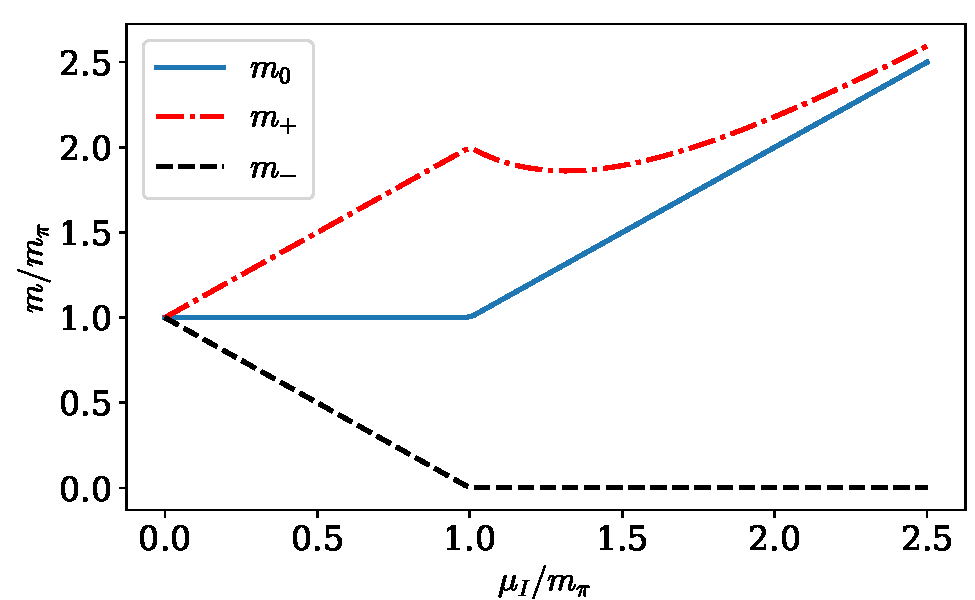
\includegraphics[width=0.7\textwidth]{figurer/numerics/masses.pdf}
    \caption{The masses of the three particles as functions of isosopin chemical potential.}
    \label{fig:masses}
\end{figure}

With these energies we can write the determinant of the inverse propagator as
\begin{equation}
    \det(D^{-1}) = (p_0^2 - E_0^2) (p_0^2 - E_+^2) (p_0^2 - E_-^2).
\end{equation}
The propagator and the inverse propagator in momentum space obey\footnote{One has to be carfull regarding the factor $i$ in the physicist's definition of propagators. It has the consequence that $D^{-1}$ is not strictly the operator inverse of the propagator $D$.}
\begin{equation}
    \sum_c D_{ac}(p)D_{cb}^{-1}(p) = i \delta_{ab}
\end{equation}
Using this, we can solve for the propagator
\begin{align}
    \notag
    D & = (- iD^{-1})^{-1} = \frac{i}{\det(D^{-1})}
    \begin{pmatrix}
        D^{-1}_{22} D^{-1}_{33}   & D^{-1}_{12}D^{-1}_{33}  & 0 \\
        -D^{-1}_{12}D^{-1}_{33}   & D^{-1}_{11}D^{-1}_{33}  & 0 \\
        0               & 0             & D^{-1}_{11}D^{-1}_{22} + (D^{-1}_{12})^2
    \end{pmatrix} \\
    \label{free pion propagator}
    & = i
    \begin{pmatrix}
        \frac{
            p^2 - m_2^2
        }
        {
            (p_0^2 - E_+^2)(p_0^2 - E_-^2)
        } 
        & \frac{
            - ip_0m_{12}
        }
        {
            (p_0^2 - E_+^2)(p_0^2 - E_-^2)
        } & 0 \\
        \frac{
            ip_0m_{12}
        }
        {
            (p_0^2 - E_+^2)(p_0^2 - E_-^2)
        }
        & \frac{
            p^2 - m_1^2
        }
        {
            (p_0^2 - E_+^2)(p_0^2 - E_-^2)
        } & 0 \\
        0 & 0 & 
        \frac{1}{p_0^2 - E_0^2}
    \end{pmatrix}.
\end{align}
